\section{Engine}
While the \langname{} compiler chain parses, validates and translates program code, the result cannot be run on its own. The engine complements the compiler by exposing a simple API that allows for the resolution of battle scenarios described in \langname{}\todo{Did I write this once already?}.

This section describes how the engine was implemented, particularly how the implementation language and compiler code generation concerns affected the final design.

\subsection{Platform}
The engine was implemented in $C++$ just like the compiler, partially because of language acclimatisation but mostly in order to simplify any bonding between the two pieces of the system. The compiler chain supports two modes of operation: compiling to engine-compatible $C++$ or initialising directly into an engine instance. This was primarily a result of design-indecision during implementation, but the platform-specific designs necessary to support the latter ended up creating a much simpler API for the prior, a net gain.

Since $C++$ has a very limited form of introspection (the dynamic\_cast and typeid keywords). Consequently a generic solution with good code re-use must make comprehensive use of polymorphism in order to approach the degree of type agnosticism that \langname{} exhibits. Thus the somewhat open-ended cross referencing allowed in \langname{} necessitates a data model wherein game objects are closely related where crossovers may happen. This referencing is apparent mostly when setting Attribute and Resource values \todo{We probably have something in syntax/semantics about RGR.Member syntax and meaning.}. The prime method of generalising this access across Primarchs was to introduce a Primarch superclass in the engine that supplied the following functionality:
\begin{description}
	\item[Meta identifiers] Run-time identifiers of objects.
	\item[Generalised values] The concept of a universal value in every run-time object.
	\item[Containment and cloning] Effective encapsulation and cloning.
\end{description}

Each is described in the following subsections.

\subsection{Meta identifiers}
Consider the \langname{} line "PhysicalDamageEffect(17 * OWNER.Strength)". \todo{Actually... this might be painfully unnecessary. The compiler's type checking should ensure valid types and their declaration, thus knowing the identity of the variable.}

Adding a human-readable string representation of a Primarch identifier together with a unique global integer identifier allows for seeking Primarch instances without knowing its type prior to retrieval. This is useful when requesting the value of the member "Power" when it is unknown whether that member is a Resource or an Attribute. While the global id is unique between container entities (two Characters do not have the same "Health" Resource), the name "Health" can be shared between them.

\subsection{Generalised value}
All Primarchs must implement a notion of a "value", representing their current state. This makes very little practical sense for Effects, Ability instance or Characters in the current language design. However, it eases the implementation of working with values for Resource and Attributes. \todo{Again, the compiler can make this obsolete.}

\subsection{Containment and cloning}
Each Primarch is in itself a potential container for other Primarchs. Several of the Primarchs contain other Primarchs, and unifying this concept across classes reduces the amount of redundant code throughout the project. Furthermore, this tree-like structure allows for a unified method for cloning an entire Character's structure for use in a parallel GameState for Behaviour calculations.

Working with an object-oriented language where references may point to the same object instance, cloning needs to be implemented with careful precision. In $C++$, copy-constructors allows for a simple syntax for copying one object into another. However, this method does not support iheritance very well. For one thing, constructors cannot be declared virtual. Furthermore, the copy-constructor must be invoked on the intended class, which may not be known at compile-time. For example, when cloning an entire GameState hierarchy, a flexible cloning method only assumes that children inherit from Primarch, nothing else. Invoking the copy-constructor on Primarch would slice the resulting object, neglecting to copy essential data - copying Resource in this way would result in a new object where the Primarch data from Resource was copied, nothing else. Consider the following example, where three classes are defined. The base class SomeClass, and two subclasses of it - DerivClass1 and DerivClass2. They each define an overridden method, get\_number(), that returns either an input number, double the number or triple the number. The following code works:

\begin{lstlisting}[language=C++]
SomeClass* a = new SomeClass(1); // a.number == 1;
std::cout << "a: " << a->get_number() << '\n'; // Prints 'a: 1'

DerivClass1* b = new DerivClass1(*a);
std::cout << "b: " << b->get_number() << '\n'; // Prints 'b: 2'

DerivClass2* c = new DerivClass2(*a);
std::cout << "c: " << c->get_number() << '\n'; // Prints 'c: 3'

c = new DerivClass2(*dynamic_cast<SomeClass*>(b));
std::cout << "c: " << c->get_number() << '\n'; // Prints 'c: 3'
\end{lstlisting}

However, it requires compile-time knowledge of the possible subclasses, a cumbersome approach that is difficult to maintain in the long run. Trying to base the code on a base class does not work when relying on a copy-constructor:

\begin{lstlisting}
std::list<SomeClass*> l;

l.push_back(new DerivClass1(*a));
l.push_back(new DerivClass2(*a));
    
// Retrieve, copy, and print. This is where the copy-constructor fail appears.
for (std::list<SomeClass*>::iterator iter = l.begin();
        iter != l.end();
        iter++)
{
    SomeClass* tmp = new SomeClass(**iter);
    std::cout << "List: " << tmp->get_number() << '\n'; // Prints 'List: 1' every time.
}
\end{lstlisting}

The benefit of polymorphism is nonexistant. It is possible to fall back to the automatically defined copy-constructor by the $C++$ compiler, but the degree to which it copies the object \emph{referenced} by a pointer or simply the pointer itself is unsure. The only effective solution is to move away from a copy-constructor to a virtual clone method that will automatically be called in the lowest subclass thanks to late dynamic binding. Assume that the classes now have a virtual clone method instead of a copy constructor. The code is identical and the "copy" parameter is now assumed implicit in the \emph{this} pointer.

\begin{lstlisting}[language=C++]
std::list<SomeClass*> l;

l.push_back(new DerivClass1(*a));
l.push_back(new DerivClass2(*a));
    
// Retrieve, copy, and print. This is where the copy-constructor fail appears.
for (std::list<SomeClass*>::iterator iter = l.begin();
        iter != l.end();
        iter++)
{
    SomeClass* tmp = (*iter)->clone(); new SomeClass(**iter);
    std::cout << "List: " << tmp->get_number() << '\n'; // Prints 'List: x', where x is the correct output from get_number()
}
\end{lstlisting}

This approach is implemented in the Primarch superclass. Without overriding it, the method will loop through all Primarchs it contains and clone them into a new Primarch instance. This is effectively a recursive procedure, traversing a Primarch collection depth-first. Subclasses are encouraged to override the method to extend it with class-specific cloning, and do so in the final reference implementation.

\subsection{Decision-making}
Characters' decision-making is defined non-deterministically. This trait means that a singular path through a game cannot be determined by a single calculation. Instead, it is necessary to calculate all possible outcomes to determine the optimal game state for a Character. To achieve this, the entire game state needed to be atomically contained and easily replicatable. From there it is a simple though cumbersome matter of a brute-force serial approach to combining abilities and valid targets to modify a temporary game state, measuring the resulting piggy value.

\begin{figure}
\missingfigure{Insert a figure demonstrating the cloning hierarchy.}
\caption{\label{figure:implementation:engine:cloning}An image giving an impression of the cloning mechanism throughout the Primarch and GameState hierarchies.}
\end{figure}

Using the deep cloning mechanism it is possible to create a completely identical copy of a game's state in memory. The set of possible actions is determined by taking each of a Character's abilities and each of that ability's valid targets. Essentially that set is a subset of $Abilities \times RelativeGlobalReferences$, typically a much smaller subset, but in all circumstances a limited one. An shortened version of this procedure can be found on Fig. \ref{figure:engine:implementation:abilitytable}.

\begin{figure}
\begin{lstlisting}[language=C++]
std::vector<Action*> *actions = this->create_actions(this->state->current_char);

float max_piggy = std::numeric_limits<float>::infinity() * -1;

for (std::vector<Action*>::iterator iter = actions->begin();
     iter != actions->end();
     iter++)
{
    Action *tmp_a = *iter;

	GameState *tmp_state = tmp_a->execute(this->state);

	float new_piggy = tmp_state->current_char->get_piggy(tmp_state);

	if (new_piggy > max_piggy)
	{
		max_piggy = new_piggy;
		this->best_action = *iter;
		this->best_state = tmp_state;
	}
}

return this->best_state;
\end{lstlisting}
%\caption{\label{figure:engine:implementation:abilitytable}An abbreviated version of AbilityTable::get\_next\_state()}
\end{figure}

Simply, this is just a loop over a set of Action objects, each defining an Ability and an RGR as a target.

\subsection{Design revisited}
The implementation described in this section caused several changes to the preliminary engine design. All Primarchs were subclassed to a super Primarch class that defined name, id and contained Primarch instances. Several extra classes were introduced to handle intermediate and interpreted values during run-time, markedly the RGR\_List, Action, ActionDefinition and EventCondition classes. They introduced a generic way to alleviate the code generation phase of the compiler, keeping it from having to generate complex blocks of code to handle variable values in cases that could be described in a general way. Ultimately, this resulted in the class diagram shown on Fig. \ref{figure:engine:implementation:new-class-diagram}.

\begin{figure}
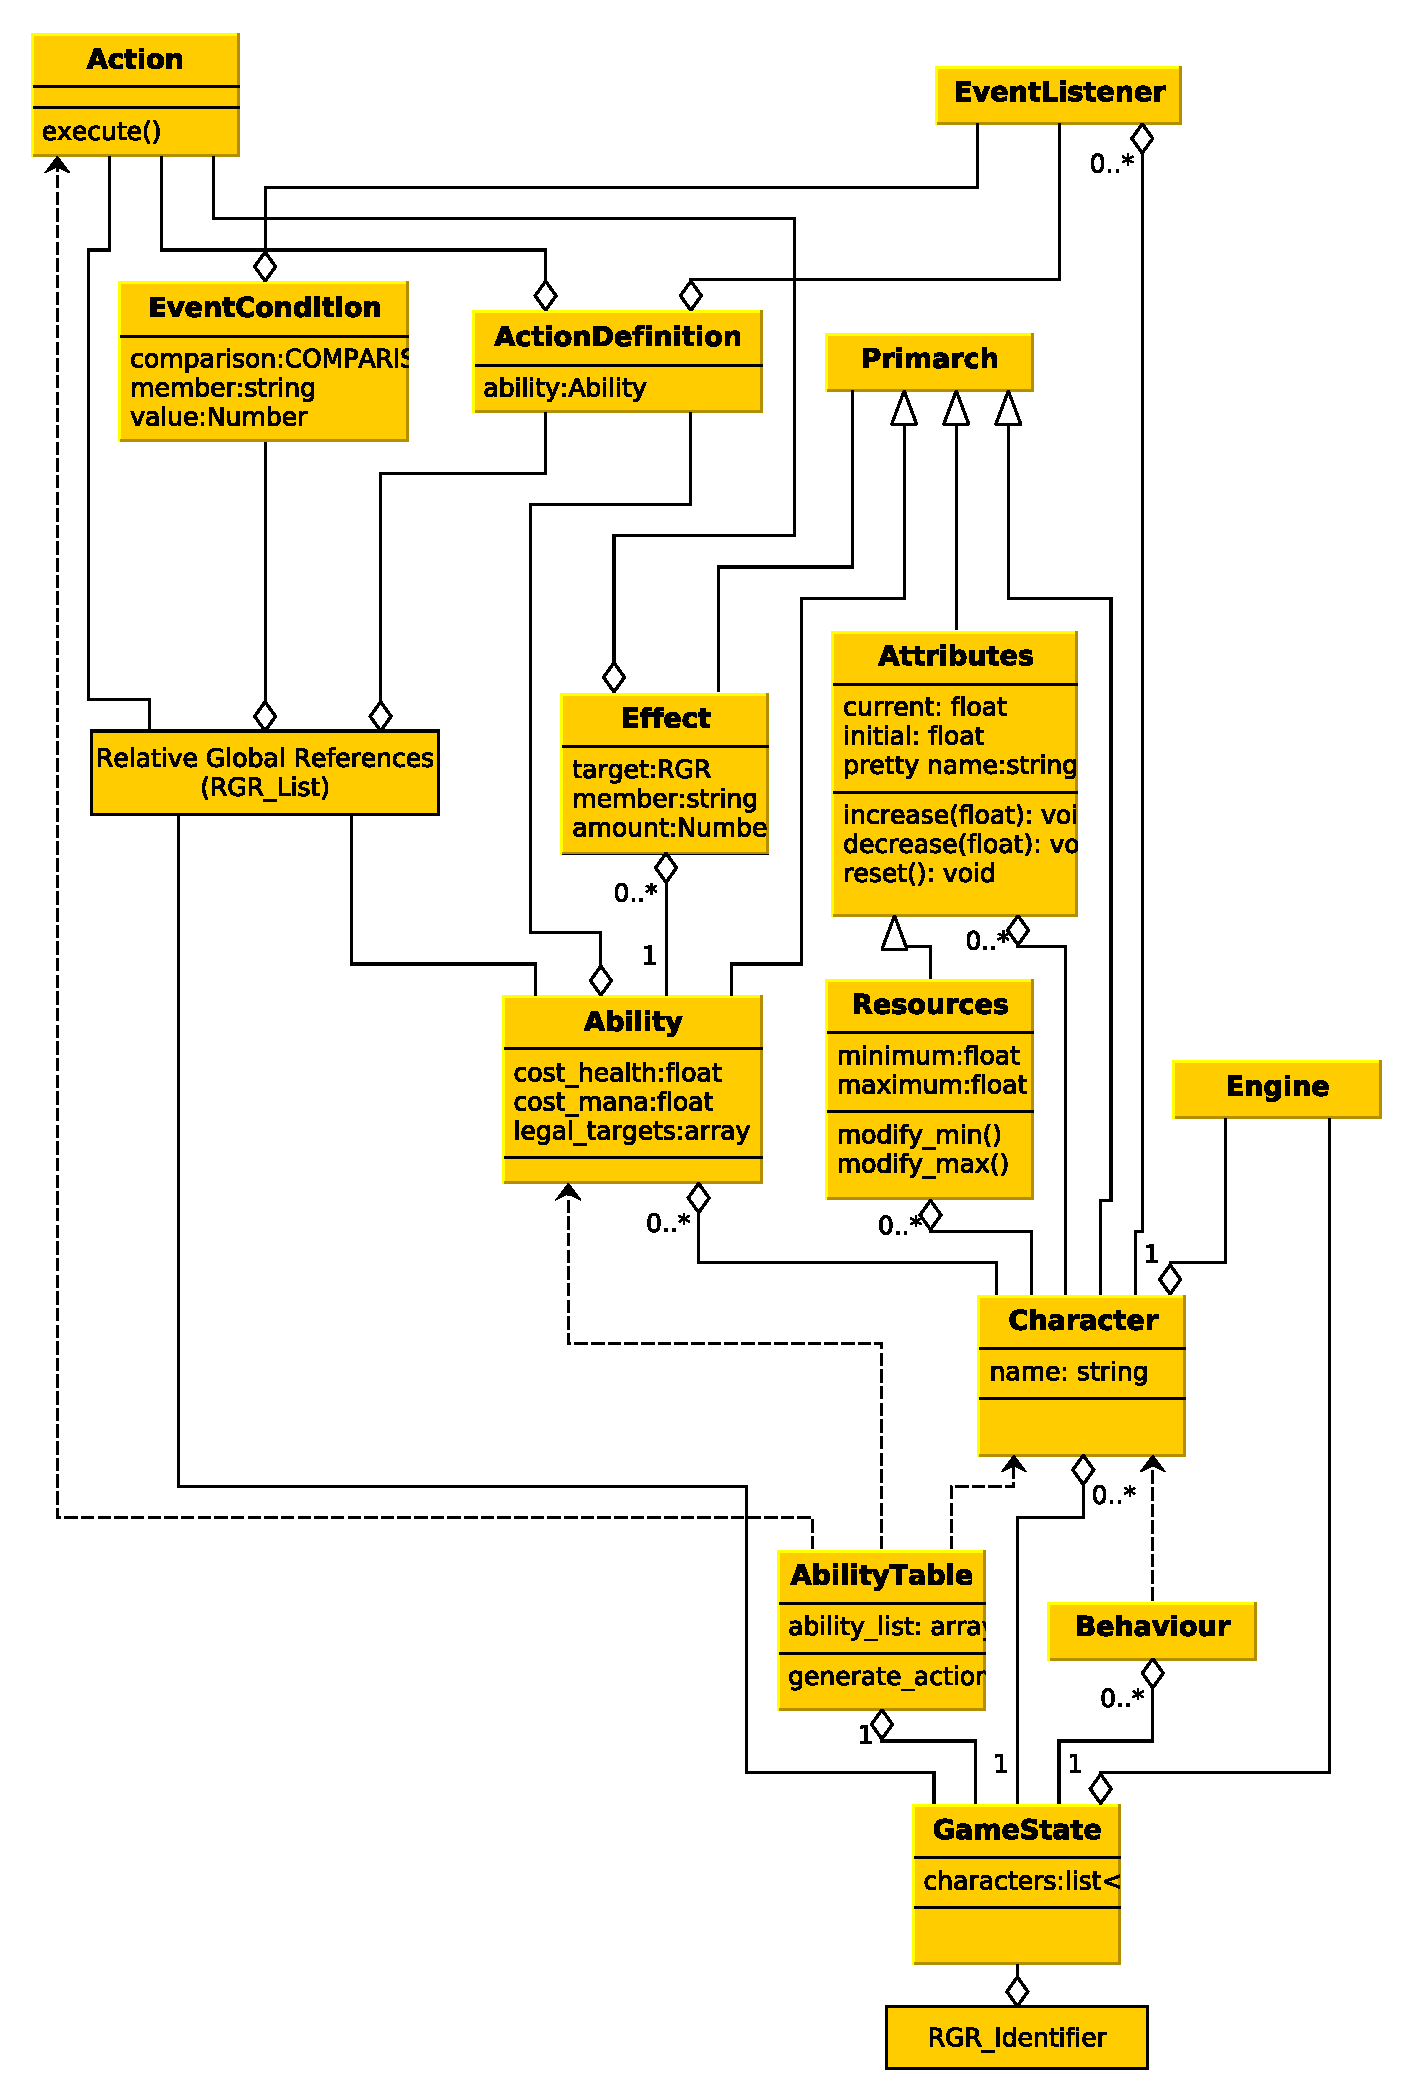
\includegraphics[width=\linewidth]{img/class_diagram_final}
\caption{\label{figure:engine:implementation:new-class-diagram}The new class diagram introduced during implementation.}
\end{figure}